% Provenance (never printed): cycle 3 "La planete Terre" (the shaping of
% landscapes: erosion, transport and deposition by running water; rivers
% from source to mouth; floods); see sources/book1/PROVENANCE.md.
% Book 1, grade 5, chapter 1.
\chapter{流水塑造大地}\label{ch:g5:water-shapes-the-land}

整夜，暴风雨敲打着学校的屋顶。
早晨，天空正在放晴，丽娜和汤姆跑向
操场后面的小溪。昨天它清澈而安静，他们能数清
河床上的\omterm{def:g3:stones-pebbles-sand:pebble}{卵石}。今天它变宽了，水流湍急，呈棕色，颜色像
牛奶巧克力。水里挟带着树枝、树叶，还有一些
他们一粒一粒都看不清的东西：泥和沙，它们是从两岸和上游
田地里冲刷下来的。

“这些泥要流到哪里去？”汤姆问。向下游，每过一分钟就更远一点。
溪水正把土地一粒一粒地带走。在本章中，
我们将追踪这些颗粒，从它们的母岩，
直到它们\omterm{def:g5:water-shapes-the-land:deposition}{沉积}下来的地方。

\begin{omfigure}
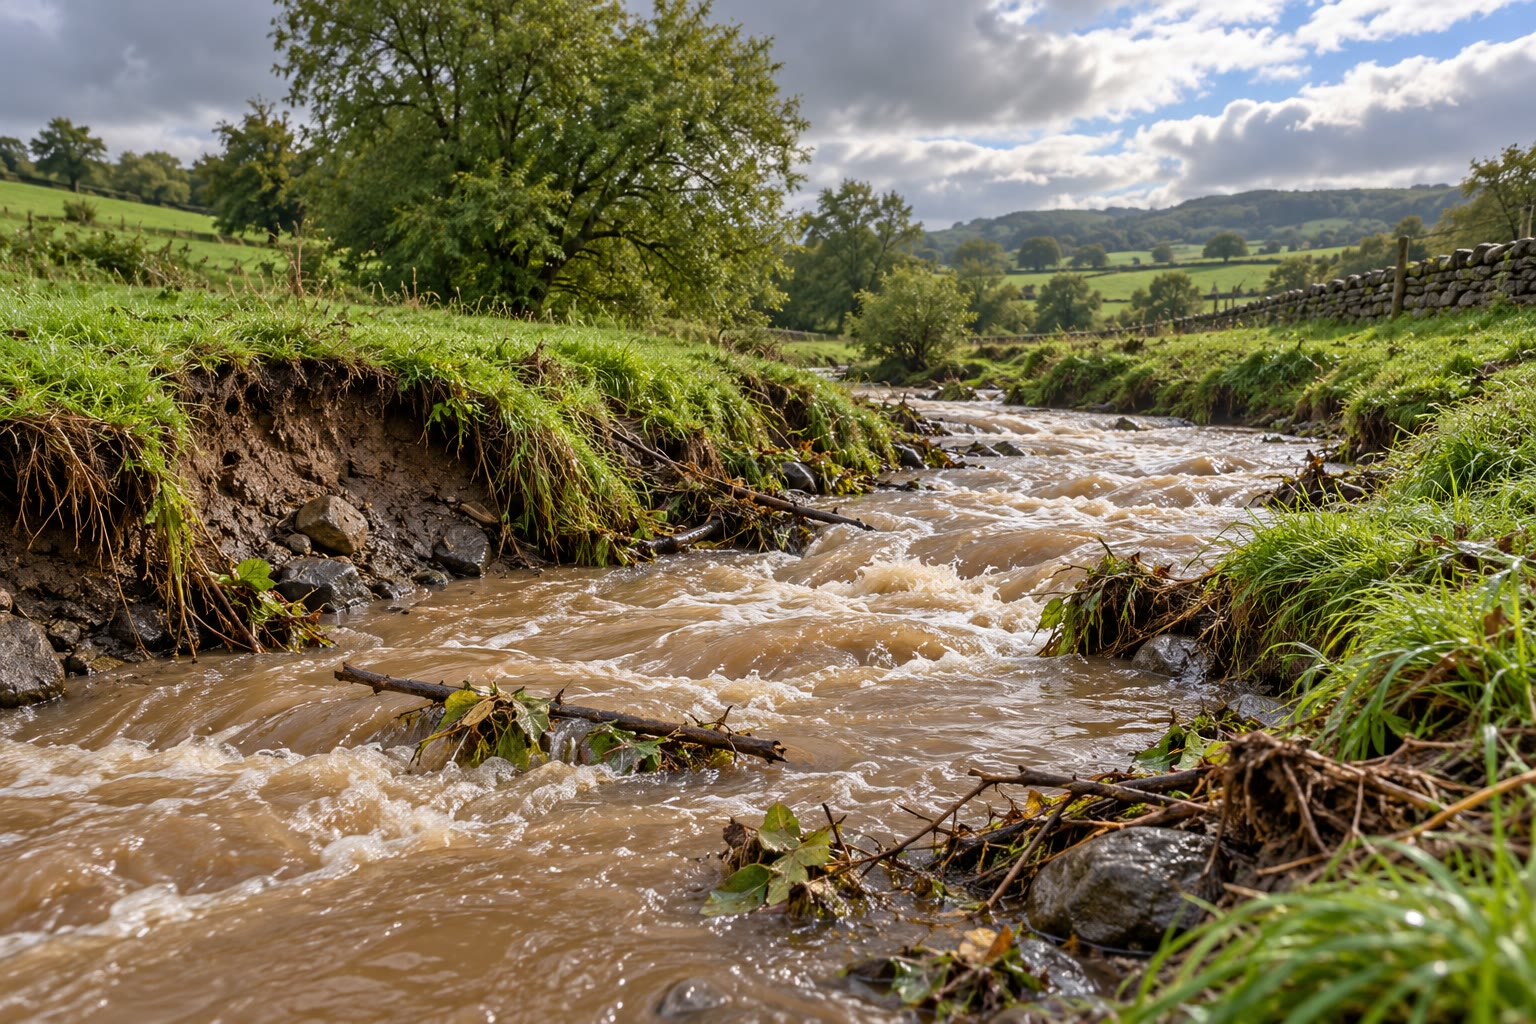
\includegraphics[width=0.5\linewidth]{images/book1/ai/g5-brown-stream.jpg}

{\small 暴风雨过后的早晨，一条小溪：水因
所携带的\omterm{def:g3:stones-pebbles-sand:sand}{泥沙}而呈棕色。}
\end{omfigure}

\begin{recall}
\omterm{def:g3:stones-pebbles-sand:rock}{岩石}是地球上坚硬的物质；打碎后便得到石块、
被水磨圆的\omterm{def:g3:stones-pebbles-sand:pebble}{卵石}、颗粒能用肉眼一粒一粒看清的沙，以及
颗粒太小、看不清的泥（见\cref{ch:g3:stones-pebbles-sand}）。\omterm{def:g1:landscapes-around-us:water}{河流}
总是沿着长长的河道流动，从较高的地方
流向\omterm{def:g1:landscapes-around-us:water}{湖泊}或大海（见\cref{ch:g1:landscapes-around-us}）。落在
陆地上的雨水流入溪流和\omterm{def:g1:landscapes-around-us:water}{河流}，再把水
带回大海（见\cref{ch:g2:water-on-earth}）。
\end{recall}

\section{岩石在原地破碎}

即使是最坚硬的\omterm{def:g3:stones-pebbles-sand:rock}{岩石}，也不会永远存在。暴露在外的\omterm{def:g3:stones-pebbles-sand:rock}{岩石}，
在阳光、雨水和霜冻的作用下，会慢慢开裂、碎裂。

\begin{definition}[风化]\label{def:g5:water-shapes-the-land:weathering}
\emph{风化}\index{风化}是\omterm{def:g3:stones-pebbles-sand:rock}{岩石}在原地缓慢破碎的过程，
破碎的原因包括霜冻、水、植物根系以及冷热变化。
\omterm{def:g3:stones-pebbles-sand:rock}{岩石}被破碎成许多小块，但碎块仍留在原地。
\end{definition}

霜冻是\omterm{def:g5:water-shapes-the-land:weathering}{风化}作用中最有力的手段之一。雨水渗入
\omterm{def:g3:stones-pebbles-sand:rock}{岩石}中细小的裂缝。寒冷的夜晚，雨水结冰，水结冰时
体积会稍稍增大：冰挤压裂缝的两壁，
使裂缝略微张开。第二天冰融化，更多的水渗入，
到了下一个夜晚又结冰。经过多个冬天，一块
\omterm{def:g3:stones-pebbles-sand:rock}{岩石}终于脱落。

\begin{omfigure}
\begin{tikzpicture}[x=1cm, y=1cm, font=\scriptsize]
  \foreach \i/\t in {0/{1. 雨水渗进 \\裂缝。},
                     4.3/{2. 夜里水结成冰：\\冰把裂缝 \\撑得更宽。},
                     8.6/{3. 许多个冬天后，\\一块岩石脱落。}} {
    \begin{scope}[xshift=\i cm]
      \fill[gray!35] (0,0) rectangle (3.4,2.6);
      \draw[gray!60!black] (0,2.6) -- (3.4,2.6);
      \node[align=center, anchor=north] at (1.7,-0.15) {\t};
    \end{scope}
  }
  % panel 1: thin crack with water
  \fill[white] (1.55,2.6) -- (1.75,0.9) -- (1.85,2.6) -- cycle;
  \fill[blue!45] (1.6,2.2) -- (1.75,0.9) -- (1.83,2.2) -- cycle;
  \draw[gray!60!black] (1.55,2.6) -- (1.75,0.9) -- (1.85,2.6);
  \foreach \x in {1.3,1.7,2.1} \draw[blue!60, ->] (\x,3.3) -- (\x+0.05,2.8);
  \node[blue!60!black] at (0.6,3.1) {雨水};
  % panel 2: wider crack with ice
  \begin{scope}[xshift=4.3cm]
    \fill[white] (1.45,2.6) -- (1.75,0.75) -- (1.98,2.6) -- cycle;
    \fill[cyan!15] (1.5,2.3) -- (1.75,0.75) -- (1.94,2.3) -- cycle;
    \draw[cyan!50!black] (1.5,2.3) -- (1.75,0.75) -- (1.94,2.3) -- cycle;
    \draw[gray!60!black] (1.45,2.6) -- (1.75,0.75) -- (1.98,2.6);
    \draw[red!70!black, thick, <-] (1.05,1.9) -- (1.5,1.9);
    \draw[red!70!black, thick, ->] (1.98,1.9) -- (2.45,1.9);
    \node[cyan!40!black] at (1.72,3.0) {冰};
  \end{scope}
  % panel 3: broken block
  \begin{scope}[xshift=8.6cm]
    \fill[white] (1.35,2.6) -- (1.75,0.6) -- (3.4,0.6) -- (3.4,2.6) -- cycle;
    \draw[gray!60!black] (1.35,2.6) -- (1.75,0.6) -- (3.4,0.6);
    \fill[gray!35, draw=gray!60!black, rotate around={-25:(2.9,0.3)}]
      (2.3,0.3) -- (2.4,1.4) -- (3.5,1.35) -- (3.4,0.3) -- cycle;
    \draw[gray!60!black, ->] (2.6,2.2) to[bend left=20] (3.0,1.5);
  \end{scope}
\end{tikzpicture}

{\small 霜冻使\omterm{def:g3:stones-pebbles-sand:rock}{岩石}破碎。每个结霜的夜晚，裂缝中的冰都会向外挤压一点；
经过多个冬天，裂缝宽到足以让一块\omterm{def:g3:stones-pebbles-sand:rock}{岩石}
脱落。}
\end{omfigure}

在高山上一座裸露的岩壁脚下，被霜冻震落的碎块
滑落、翻滚，堆积成一道布满棱角石块的斜坡。
它们尚未被磨圆：还没有水流把它们冲刷过。

\begin{omfigure}
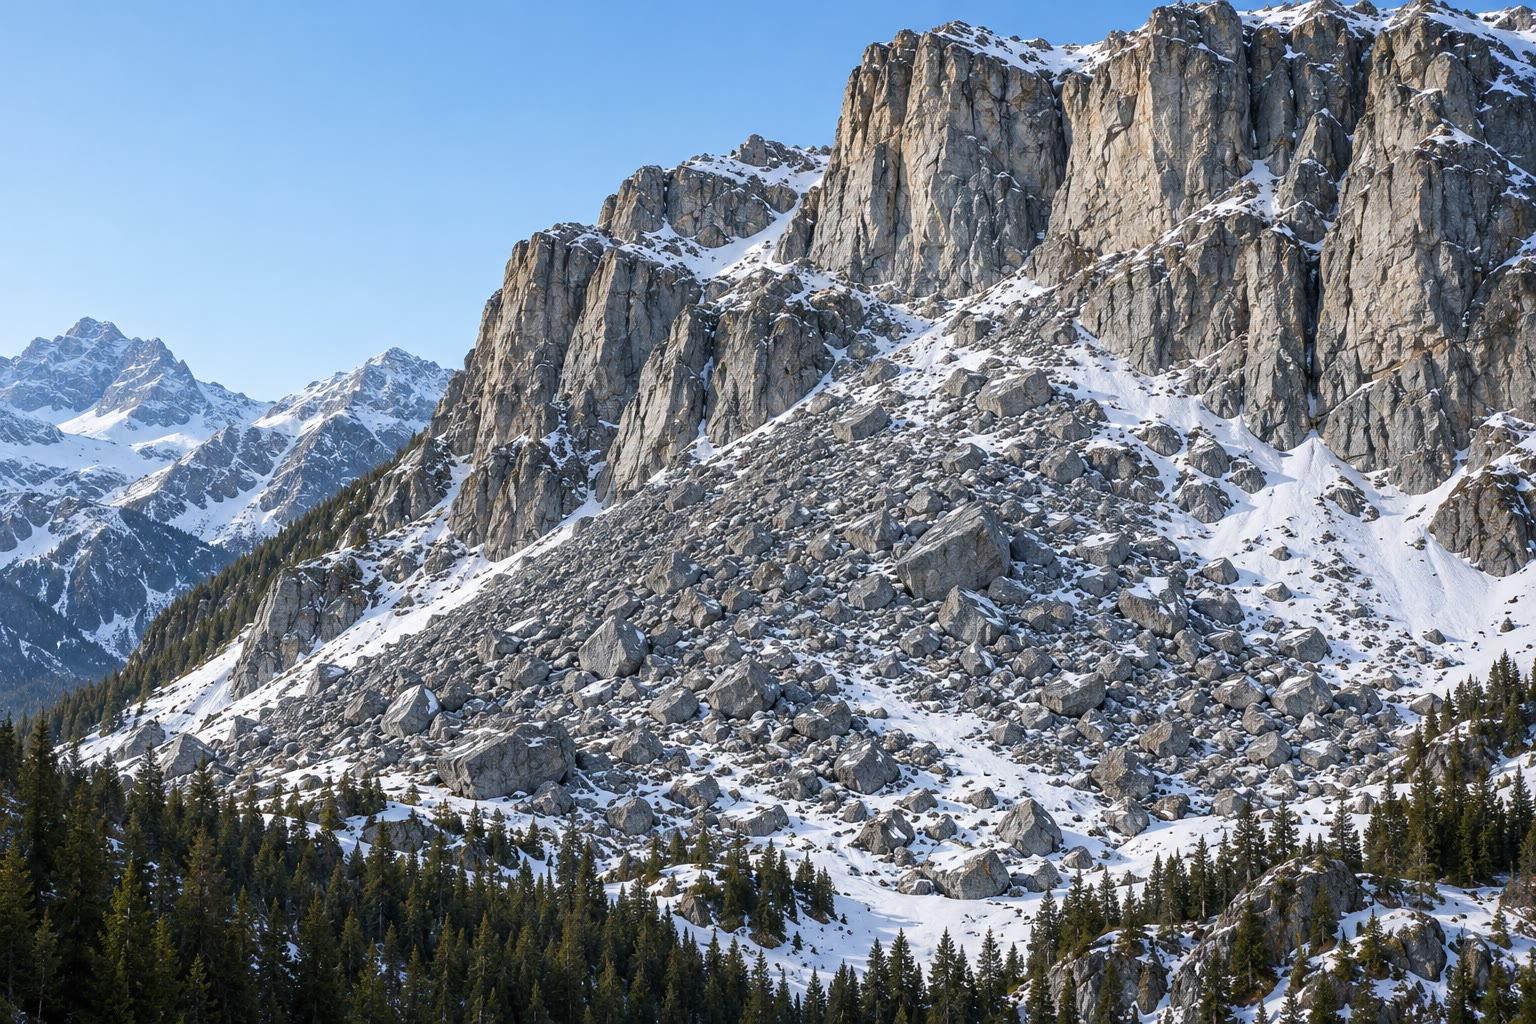
\includegraphics[width=0.5\linewidth]{images/book1/ai/g5-frost-scree.jpg}

{\small 山崖脚下，被霜冻震落的棱角分明的石块坡，
从\omterm{def:g1:landscapes-around-us:landform}{山谷}对面望去。}
\end{omfigure}

植物也起作用。一棵树的根钻进裂缝，随着
年复一年地长粗，像一个缓慢的楔子把\omterm{def:g3:stones-pebbles-sand:rock}{岩石}劈开。雨水本身
也会慢慢软化某些\omterm{def:g3:stones-pebbles-sand:rock}{岩石}，使其变成黏土和沙：
土壤正是这样获得它的矿物颗粒的。

\section{水搬运碎屑}

\omterm{def:g3:stones-pebbles-sand:rock}{岩石}一旦破碎，碎屑就能移动。总得有什么东西把它们搬走。

\begin{definition}[侵蚀]\label{def:g5:water-shapes-the-land:erosion}
\emph{侵蚀}\index{侵蚀}是陆地被磨损、
\omterm{def:g3:stones-pebbles-sand:rock}{岩石}碎屑被搬运走的过程，
其中以流水的作用为主，也包括风、冰和海浪的作用。
\end{definition}

流水做了大部分的工作。雨水把土壤和颗粒冲下
山坡，汇入溪流；溪流又从自己的河岸上冲走更多物质，
就像暴风雨过后汤姆和莉娜的小溪那样。水流越快，
能搬运的物质就越多，能移动的碎块也越大：
平静的小溪只能搬运细泥；涨水的溪流甚至能把\omterm{def:g3:stones-pebbles-sand:pebble}{卵石}
乃至巨石沿河床滚动。

石头在搬运途中相互碰撞，也与河床碰撞。
棱角被磨掉，变成圆滑的\omterm{def:g3:stones-pebbles-sand:pebble}{卵石}，然后越变越小，
最终成为沙和泥。

在干燥的地方，风也做同样的工作，那里没有东西固定\omterm{def:g3:stones-pebbles-sand:sand}{沙子}：
风把沙吹成沙丘。冰在山区和极地附近，
在巨大的重量下拖动石块。\omterm{def:g1:landscapes-around-us:water}{海岸}上，海浪拍打悬崖，
并使海滩上的\omterm{def:g3:stones-pebbles-sand:pebble}{卵石}来回滚动。

\begin{remark}[有多少？]\label{rem:g5:water-shapes-the-land:how-much}
全世界所有\omterm{def:g1:landscapes-around-us:water}{河流}每年输入大海的
\omterm{def:g3:stones-pebbles-sand:sand}{泥沙}合计超过 120 亿吨，
相当于每月约 10 亿吨。
% ledger: syvitski:modern-flux
\end{remark}

\section{水把碎屑沉积下来}

\omterm{def:g1:landscapes-around-us:water}{河流}不能永远搬运它的负荷。流速减慢之处，
\omterm{def:g1:landscapes-around-us:water}{河流}已没有力量搬动最大的颗粒，它们便\omterm{def:g5:water-shapes-the-land:deposition}{沉积}在河床上。

\begin{definition}[沉积]\label{def:g5:water-shapes-the-land:deposition}
\emph{沉积}\index{沉积}是\omterm{def:g3:stones-pebbles-sand:rock}{岩石}碎屑被水、风或冰搬运后，
在速度减慢并停止的地方堆积下来的过程。
\end{definition}

最重的碎屑最先沉降：\omterm{def:g3:stones-pebbles-sand:pebble}{卵石}在水流稍有减缓的地方沉落，
沙在流速减缓更多的地方沉落，细泥只在水几乎静止的地方
即\omterm{def:g1:landscapes-around-us:water}{湖泊}或大海中\omterm{def:g5:water-shapes-the-land:deposition}{沉积}。这就是河床在山区多\omterm{def:g3:stones-pebbles-sand:pebble}{卵石}、
靠近大海处多沙或泥的原因。

\omterm{def:g5:water-shapes-the-land:weathering}{风化}、\omterm{def:g5:water-shapes-the-land:erosion}{侵蚀}和\omterm{def:g5:water-shapes-the-land:deposition}{沉积}是同一段漫长旅程的三个阶段：
\omterm{def:g3:stones-pebbles-sand:rock}{岩石}在原地被破碎，碎屑被搬走，并且
在别处\omterm{def:g5:water-shapes-the-land:deposition}{沉积}下来。流水就这样一粒一粒地搬动\omterm{def:g4:world-physical-map:range}{山脉}，
把它们带到\omterm{def:g1:landscapes-around-us:landform}{平原}，最终送入大海。

\begin{method}[说出水的作用]\label{met:g5:water-shapes-the-land:naming}
要说出图画或故事中\omterm{def:g3:stones-pebbles-sand:rock}{岩石}正在发生的变化，
可以问以下三个问题：
\begin{enumerate}
  \item \omterm{def:g3:stones-pebbles-sand:rock}{岩石}是否被破碎，但碎屑仍留在原处？
        这是\emph{\omterm{def:g5:water-shapes-the-land:weathering}{风化}}。
  \item 碎屑是否被磨损并被搬走？这是
        \emph{\omterm{def:g5:water-shapes-the-land:erosion}{侵蚀}}。
  \item 碎屑是否正在沉落并堆积起来？这是
        \emph{\omterm{def:g5:water-shapes-the-land:deposition}{沉积}}。
\end{enumerate}
\end{method}

\begin{example}[暴风雨过后的小溪]\label{ex:g5:water-shapes-the-land:stream}
汤姆和莉娜小溪中浑浊的水，携带着从河岸冲刷下来的泥：
这是\omterm{def:g5:water-shapes-the-land:erosion}{侵蚀}。一周后，小溪重新变清，
操场尽头平静的水塘底部覆盖着一薄层泥：
这是\omterm{def:g5:water-shapes-the-land:deposition}{沉积}。
\end{example}

\section{一条河从源头到河口}

每条\omterm{def:g1:landscapes-around-us:water}{河流}都有开端和终点。

\begin{definition}[源头、河口和支流]\label{def:g5:water-shapes-the-land:source-mouth}
\omterm{def:g1:landscapes-around-us:water}{河流}的\emph{源头}\index{源头（河流）}是它开始的地方，
可以是泉、正在融化的冰川，或是许多细小溪流发源的高处湿地。
\omterm{def:g1:landscapes-around-us:water}{河流}的\emph{河口}\index{河口（河流）}是它的终点，即河水流入
大海、\omterm{def:g1:landscapes-around-us:water}{湖泊}或另一条更大的\omterm{def:g1:landscapes-around-us:water}{河流}的地方。
一条较小的\omterm{def:g1:landscapes-around-us:water}{河流}流入较大的\omterm{def:g1:landscapes-around-us:water}{河流}，
便是后者的\emph{支流}\index{支流}。
\end{definition}

\omterm{def:g1:landscapes-around-us:water}{河流}在流动的过程中会发生变化。我们把\omterm{def:g1:landscapes-around-us:water}{河流}的长度分为三段，
即上游、中游和下游。

\begin{omfigure}
\begin{tikzpicture}[x=1.15cm, y=1cm, font=\scriptsize]
  % ground
    \fill[brown!25] (0,-0.6) -- plot[domain=0:11, samples=60]
    (\x,{4.6*exp(-\x/2.4)}) -- (11,-0.6) -- cycle;
  % sea
  \fill[blue!20] (11,-0.6) rectangle (12.6,0.02);
  \draw[blue!70!black, line width=1.3pt] plot[domain=0.15:11, samples=60]
    (\x,{4.6*exp(-\x/2.4)});
  \draw[gray] (11,0.02) -- (12.6,0.02);
  \node[blue!50!black] at (11.9,-0.3) {海};
  % course limits
  \foreach \x in {2.6,6.6} \draw[gray, dashed] (\x,-0.6) -- (\x,5.4);
  \node[align=center, anchor=north] at (1.3,6.3) {\textbf{上游}\\坡陡、水急，\\V 形山谷};
  \node[align=center, anchor=north] at (4.6,6.3) {\textbf{中游}\\坡度较缓，\\曲流};
  \node[align=center, anchor=north] at (8.8,6.3) {\textbf{下游}\\地势平缓、流速慢，\\宽阔河漫滩};
  % source and mouth
  \fill[blue!70!black] (0.15,{4.6*exp(-0.15/2.4)}) circle (2pt);
  \node[anchor=east] at (0.05,3.7) {源头};
  \draw[->] (0.05,3.75) -- (0.12,4.15);
  \node[anchor=south] at (11.4,0.75) {河口};
  \draw[->] (11.4,0.75) -- (11.05,0.15);
  % grain sizes
  \node[anchor=north, align=center, text=brown!50!black] at (1.3,-0.7) {巨石、卵石};
  \node[anchor=north, align=center, text=brown!50!black] at (4.6,-0.7) {卵石、沙};
  \node[anchor=north, align=center, text=brown!50!black] at (8.8,-0.7) {沙、泥};
  \node[anchor=north, align=center, text=brown!50!black] at (11.8,-0.7) {泥};
\end{tikzpicture}

{\small \omterm{def:g1:landscapes-around-us:water}{河流}的纵剖面，从\omterm{def:g5:water-shapes-the-land:source-mouth}{源头}到\omterm{def:g5:water-shapes-the-land:source-mouth}{河口}（
高度被大幅拉伸）。下方：河床上的\omterm{def:g5:water-shapes-the-land:deposition}{沉积}物。}
\end{omfigure}

\omterm{def:g1:landscapes-around-us:water}{河流}在\emph{上游}时，位于山区，还很年轻，坡度陡峭。
水流湍急，沿河床滚动巨石，并向下切入\omterm{def:g3:stones-pebbles-sand:rock}{岩石}。
它切出一条狭窄的\omterm{def:g1:landscapes-around-us:landform}{山谷}，两侧陡峭，
形如字母 V。

在\emph{中游}，坡度变缓。\omterm{def:g1:landscapes-around-us:water}{河流}
左右大幅摆动，形成大弯。

\begin{definition}[曲流]\label{def:g5:water-shapes-the-land:meander}
称\emph{曲流}\index{曲流}为\omterm{def:g1:landscapes-around-us:water}{河流}的一个弯环，它
蜿蜒穿过平坦的谷底。
\end{definition}

\omterm{def:g5:water-shapes-the-land:meander}{曲流}并非静止不动，而是在移动。在每个弯道的外侧，
水流快而深，冲刷河岸，使岸壁变成一个小
悬崖。在弯道的内侧，水流缓慢，\omterm{def:g5:water-shapes-the-land:deposition}{沉积}下沙和
\omterm{def:g3:stones-pebbles-sand:pebble}{砾石}，形成平缓的河滩。年复一年，外岸被
\omterm{def:g5:water-shapes-the-land:erosion}{侵蚀}后退，内侧河滩不断扩大，弯环也越摆越宽。

\begin{omfigure}
\begin{tikzpicture}[x=1cm, y=1cm, font=\scriptsize]
  % ---- map view ----
  \fill[green!12] (-0.4,-2.5) rectangle (6.4,2.5);
  % sand on the inner banks (drawn first, the river covers its edge)
  \foreach \c/\s in {1/1, 3/-1, 5/1}
    \fill[yellow!50!orange!45] (\c-0.6,\s*0.5) .. controls (\c,\s*1.5) ..
      (\c+0.6,\s*0.5) .. controls (\c,\s*0.75) .. cycle;
  % the river
  \draw[blue!35, line width=11pt] plot[domain=-0.3:6.3, samples=90]
    (\x,{1.25*sin(\x*90)});
  \draw[blue!70!black, ->, thick] plot[domain=1.6:2.4, samples=10]
    (\x,{1.25*sin(\x*90)});
  \draw[blue!70!black, ->, thick] plot[domain=3.6:4.4, samples=10]
    (\x,{1.25*sin(\x*90)});
  % erosion on the outer banks
  \foreach \c/\s in {1/1, 3/-1, 5/1}
    \foreach \d in {-0.3,0,0.3}
      \draw[red!70!black, thick, ->] (\c+\d,{\s*(1.25*cos(\d*90)+0.22)})
        -- (\c+\d,{\s*(1.25*cos(\d*90)+0.6)});
  \node[red!70!black] at (1,2.2) {外岸侵蚀};
  \node[red!70!black] at (3,-2.2) {外岸侵蚀};
  \node[orange!40!black, align=center] (d1) at (1,-0.55) {沉积：\\内岸};
  \node[orange!40!black, align=center] (d2) at (3,0.55) {沉积：\\内岸};
  \draw[orange!40!black] (d1.north) -- (1,0.7);
  \draw[orange!40!black] (d2.south) -- (3,-0.7);
  \draw[gray!50!black, dashed] (5,0.15) -- (5,2.3);
  \node[gray!50!black, anchor=north] at (5,0.15) {剖面};
  \node[gray!50!black, anchor=east] at (4.95,0.35) {A};
  \node[gray!50!black, anchor=east] at (4.95,2.15) {B};
  \node[anchor=west] at (6.5,0) {平面图};
  % ---- cut ----
  \begin{scope}[yshift=-4.1cm, xscale=0.77]
    \fill[brown!25] (-0.4,-1.3) -- (-0.4,0.9) -- (1,0.9) -- (3.6,-0.8)
      .. controls (4.4,-1.05) .. (4.9,-0.9) -- (5.1,0.9) -- (8.4,0.9)
      -- (8.4,-1.3) -- cycle;
    \fill[blue!25] (1.75,0.4) -- (3.6,-0.8) .. controls (4.4,-1.05) .. (4.9,-0.9)
      -- (5.04,0.4) -- cycle;
    \fill[yellow!50!orange!40] (1,0.9) -- (3.6,-0.8) -- (2.6,-0.8) -- cycle;
    \draw[gray!60!black] (-0.4,0.9) -- (1,0.9) -- (3.6,-0.8)
      .. controls (4.4,-1.05) .. (4.9,-0.9) -- (5.1,0.9) -- (8.4,0.9);
    \draw[blue!60!black] (1.75,0.4) -- (5.04,0.4);
    \node[orange!40!black, align=center] at (0.9,-0.4) {内岸：\\水流缓慢，\\沙质河滩};
    \node[red!70!black, align=center, anchor=west] at (5.3,-0.3) {外岸：\\水流快而深，\\一小段悬崖};
    \draw[red!70!black, thick, ->] (4.6,-0.2) -- (5.0,-0.2);
    \node[gray!50!black, anchor=south] at (-0.2,0.9) {A};
    \node[gray!50!black, anchor=south] at (8.2,0.9) {B};
    \node[anchor=west] at (8.45,0) {剖面 A--B};
  \end{scope}
\end{tikzpicture}

{\small 从上方看到的\omterm{def:g5:water-shapes-the-land:meander}{曲流}，以及沿虚线 A--B 所作的剖面。
水流冲刷每个弯道的外岸，并在内岸\omterm{def:g5:water-shapes-the-land:deposition}{沉积}沙：
弯环因此缓慢移动。}
\end{omfigure}

有时两个弯环靠得很近，\omterm{def:g5:water-shapes-the-land:flood}{洪水}期间，\omterm{def:g1:landscapes-around-us:water}{河流}
冲破它们之间狭窄的陆颈，走上捷径。原来的
弯环被遗留下来，形成一个弯曲的\omterm{def:g1:landscapes-around-us:water}{湖泊}。

\begin{omfigure}
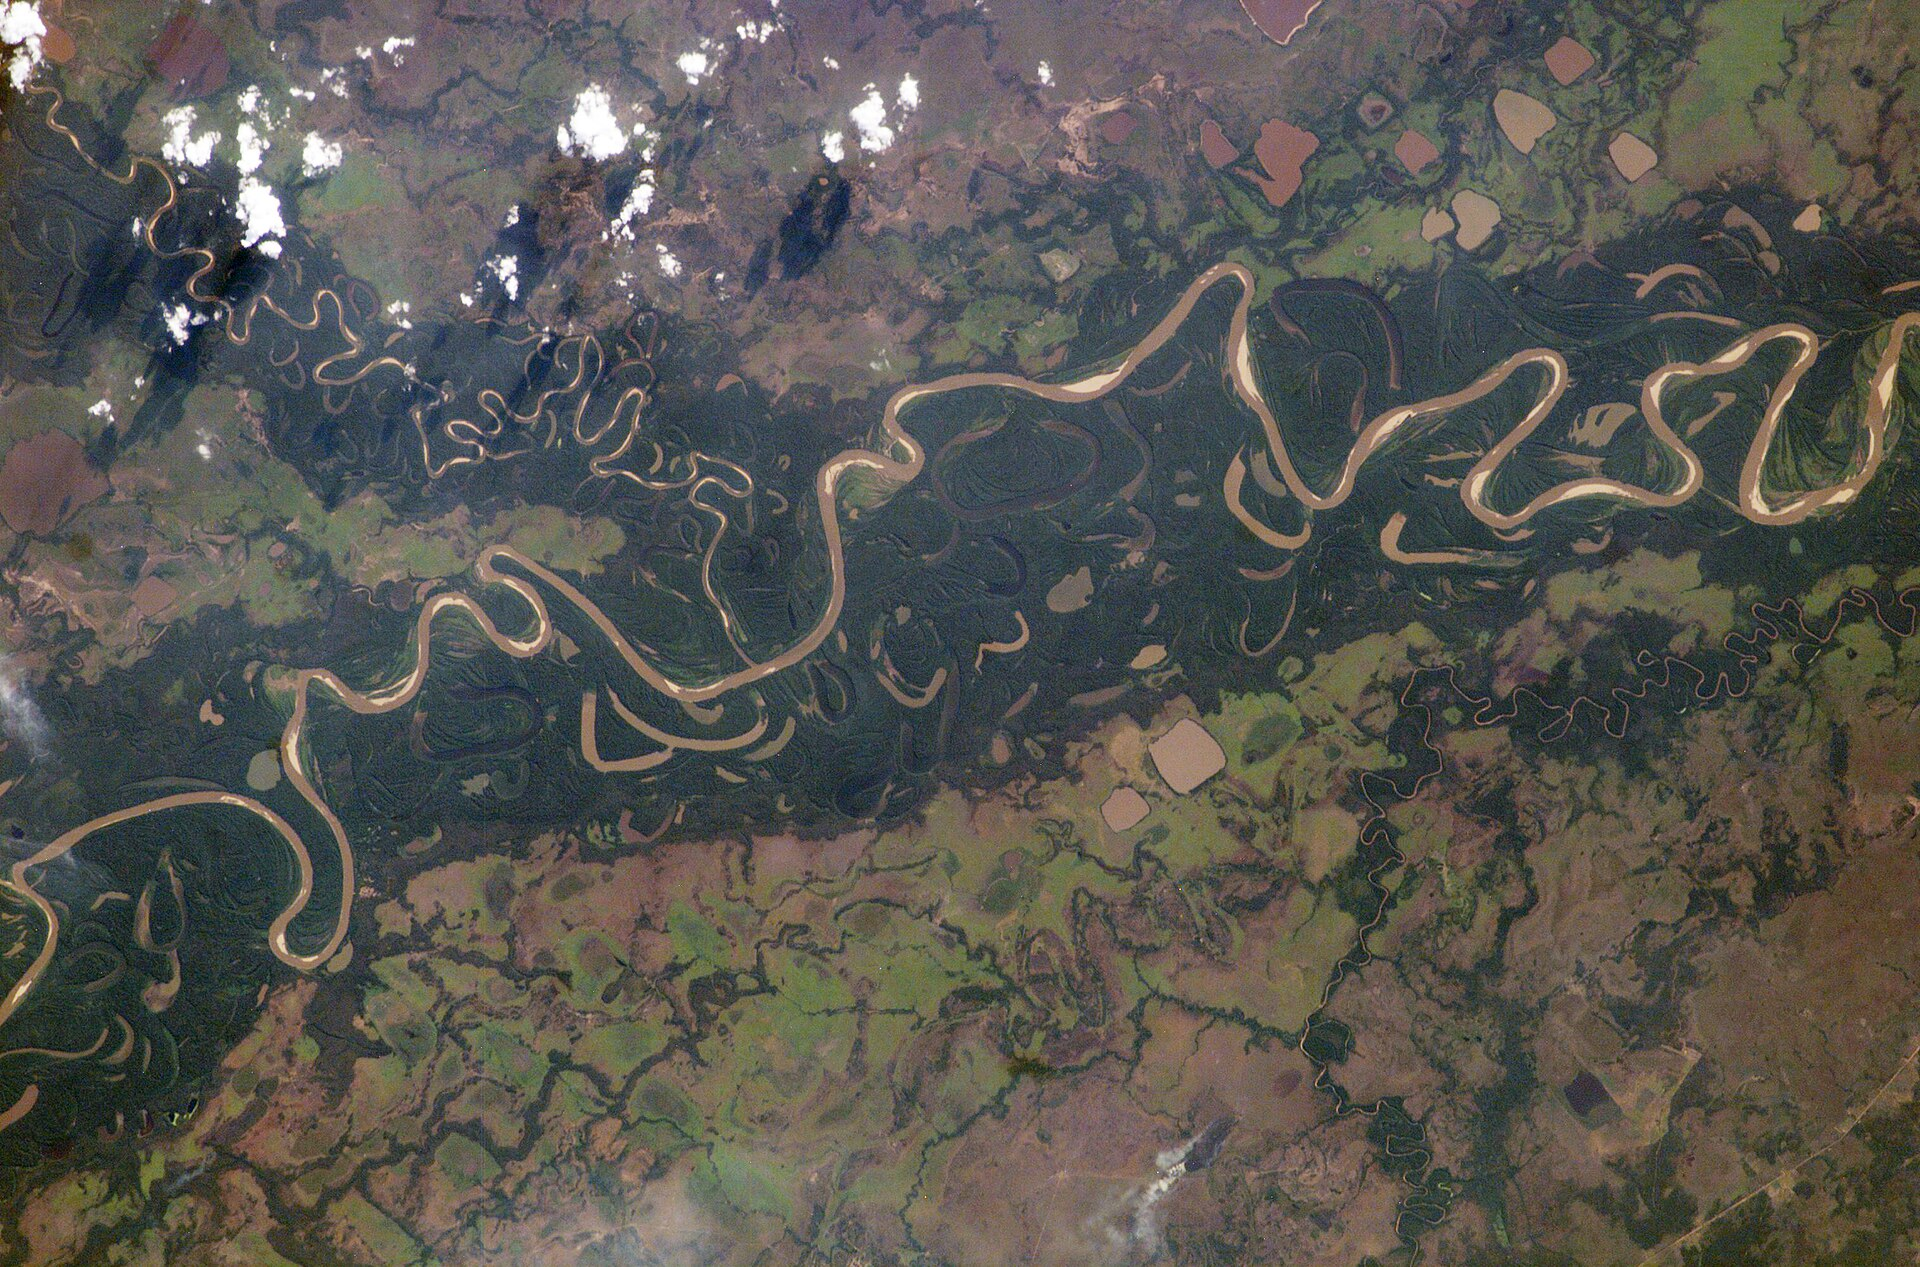
\includegraphics[width=0.52\linewidth]{images/book1/g5-mamore-meanders.jpg}

{\small 马莫雷河，位于南美洲玻利维亚的低地，从
国际空间站望去。棕色的\omterm{def:g1:landscapes-around-us:water}{河流}在森林中蜿蜒形成\omterm{def:g5:water-shapes-the-land:meander}{曲流}。
照片：NASA（公有领域）。}\label{fig:g5:water-shapes-the-land:mamore}
% ledger: nasa:mamore-meanders
\end{omfigure}

\omterm{def:g1:landscapes-around-us:water}{河流}在\emph{下游}处，地势几乎平坦。河水
缓慢流过宽阔平坦的谷底，谷底由\omterm{def:g1:landscapes-around-us:water}{河流}自身
长期\omterm{def:g5:water-shapes-the-land:deposition}{沉积}的泥和沙构成。

\begin{omfigure}
\begin{tikzpicture}[x=1cm, y=1cm, font=\scriptsize]
  % V-shaped valley
  \fill[gray!30] (0,0) -- (0,2.6) -- (0.5,2.6) -- (2.3,0.45) -- (2.7,0.45)
    -- (4.5,2.6) -- (5,2.6) -- (5,0) -- cycle;
  \fill[blue!35] (2.3,0.45) -- (2.4,0.25) -- (2.6,0.25) -- (2.7,0.45) -- cycle;
  \draw[gray!60!black] (0,2.6) -- (0.5,2.6) -- (2.3,0.45) -- (2.4,0.25)
    -- (2.6,0.25) -- (2.7,0.45) -- (4.5,2.6) -- (5,2.6);
  \draw[red!70!black, thick, ->] (2.5,1.9) -- (2.5,0.6);
  \node[red!70!black, anchor=south] at (2.5,1.9) {向下切割};
  \node[align=center, anchor=north] at (2.5,-0.1) {上游：\\狭窄的 V 形山谷};
  % floodplain
  \begin{scope}[xshift=6cm]
    \fill[gray!30] (0,0) -- (0,2.6) -- (0.6,2.6) -- (1.3,0.9) -- (5.7,0.9)
      -- (6.4,2.6) -- (7,2.6) -- (7,0) -- cycle;
    \fill[brown!25] (1.3,0.9) -- (1.55,0.3) -- (5.45,0.3) -- (5.7,0.9) -- cycle;
    \fill[blue!35] (3.1,0.9) -- (3.25,0.62) -- (3.85,0.62) -- (4,0.9) -- cycle;
    \draw[gray!60!black] (0,2.6) -- (0.6,2.6) -- (1.3,0.9) -- (3.1,0.9)
      -- (3.25,0.62) -- (3.85,0.62) -- (4,0.9) -- (5.7,0.9) -- (6.4,2.6) -- (7,2.6);
    \draw[blue!60!black, dashed] (1.22,1.1) -- (5.78,1.1);
    \node[blue!50!black, anchor=south] at (2.0,1.12) {洪水时};
    \node[brown!50!black] at (2.2,0.55) {泥和沙};
    \draw[<->] (1.3,1.75) -- (5.7,1.75);
    \node[anchor=south] at (3.5,1.75) {河漫滩};
    \node[align=center, anchor=north] at (3.5,-0.1) {下游：\\宽阔平坦的谷底};
  \end{scope}
\end{tikzpicture}

{\small \omterm{def:g1:landscapes-around-us:landform}{山谷}横切山区与海边（
比例不一）。\omterm{def:g5:water-shapes-the-land:flood}{洪水}时，\omterm{def:g1:landscapes-around-us:water}{河流}漫过整个\omterm{def:g5:water-shapes-the-land:flood}{河漫滩}。}
\end{omfigure}

最后，\omterm{def:g1:landscapes-around-us:water}{河流}抵达\omterm{def:g5:water-shapes-the-land:source-mouth}{河口}。那里的水流几乎
完全停滞，\omterm{def:g1:landscapes-around-us:water}{河流}卸下了所携带的最后一部分\omterm{def:g3:stones-pebbles-sand:sand}{泥沙}。当海浪
和潮汐的力量不足以将其全部带走时，泥和沙
逐渐堆积，新的陆地向海中延伸。

\begin{definition}[三角洲]\label{def:g5:water-shapes-the-land:delta}
\emph{三角洲}\index{三角洲}是\omterm{def:g1:landscapes-around-us:water}{河流}在\omterm{def:g5:water-shapes-the-land:source-mouth}{河口}处
由其\omterm{def:g5:water-shapes-the-land:deposition}{沉积}的泥和沙所形成的新的平坦陆地。\omterm{def:g1:landscapes-around-us:water}{河流}分成若干分支，
散布其上，常呈扇形。
\end{definition}

这一名称来自希腊字母 $\Delta$，它是一个三角形，
因为埃及尼罗河的\omterm{def:g5:water-shapes-the-land:delta}{三角洲}就是这种形状。

有些\omterm{def:g1:landscapes-around-us:water}{河流}没有\omterm{def:g5:water-shapes-the-land:delta}{三角洲}。在强浪和潮汐
将\omterm{def:g3:stones-pebbles-sand:sand}{泥沙}冲走之处，\omterm{def:g1:landscapes-around-us:water}{河流}注入一个宽阔的漏斗形\omterm{def:g5:water-shapes-the-land:source-mouth}{河口}，海水在此
随潮汐涨落进出，这种\omterm{def:g5:water-shapes-the-land:source-mouth}{河口}称为\emph{\omterm{def:g5:water-shapes-the-land:source-mouth}{河口}湾}。

\begin{omfigure}
\begin{minipage}[b]{0.55\linewidth}\centering
\begin{tikzpicture}[x=0.68cm, y=0.62cm, font=\scriptsize]
  \fill[blue!20] (-3.6,1.4) rectangle (3.6,3.6);
  \fill[green!15] (-3.6,-1.6) rectangle (3.6,1.4);
  % delta
  \fill[olive!35] (-2.6,1.4) .. controls (-2.2,2.4) and (-1,2.9)
    .. (0,3.0) .. controls (1,2.9) and (2.2,2.4) .. (2.6,1.4) -- cycle;
  \draw[gray!60!black] (-3.6,1.4) -- (-2.6,1.4) .. controls (-2.2,2.4) and
    (-1,2.9) .. (0,3.0) .. controls (1,2.9) and (2.2,2.4) .. (2.6,1.4) -- (3.6,1.4);
  \draw[gray!60!black, dashed] (-2.6,1.4) -- (2.6,1.4);
  % river and branches
  \draw[blue!60!black, line width=2pt] (0,-1.6) .. controls (0.3,-0.5) .. (0,0.9);
  \foreach \e in {-1.9,-0.9,0.2,1.2,2.0}
    \draw[blue!60!black, line width=1pt] (0,0.9) .. controls (\e*0.3,1.6) ..
      (\e,{2.95-0.3*\e*\e});
  % mud plume
  \fill[brown!30, opacity=0.5] (-1.3,3.05) .. controls (0,3.6) .. (1.3,3.0)
    .. controls (0,3.25) .. cycle;
  \node[align=center] at (-2.8,3.1) {海};
  \node[anchor=west, brown!50!black] at (1.35,3.25) {泥};
  \node[anchor=west, align=left] at (3.7,2.4) {三角洲：\\新陆地};
  \draw (3.7,2.4) -- (2.0,2.2);
  \node[anchor=west, align=left, gray!50!black] at (3.7,1.0) {旧 \\海岸};
  \draw[gray!50!black] (3.7,1.0) -- (2.3,1.4);
  \node[anchor=west] at (0.35,-1.1) {河流};
\end{tikzpicture}
\end{minipage}\hfill
\begin{minipage}[b]{0.3\linewidth}\centering
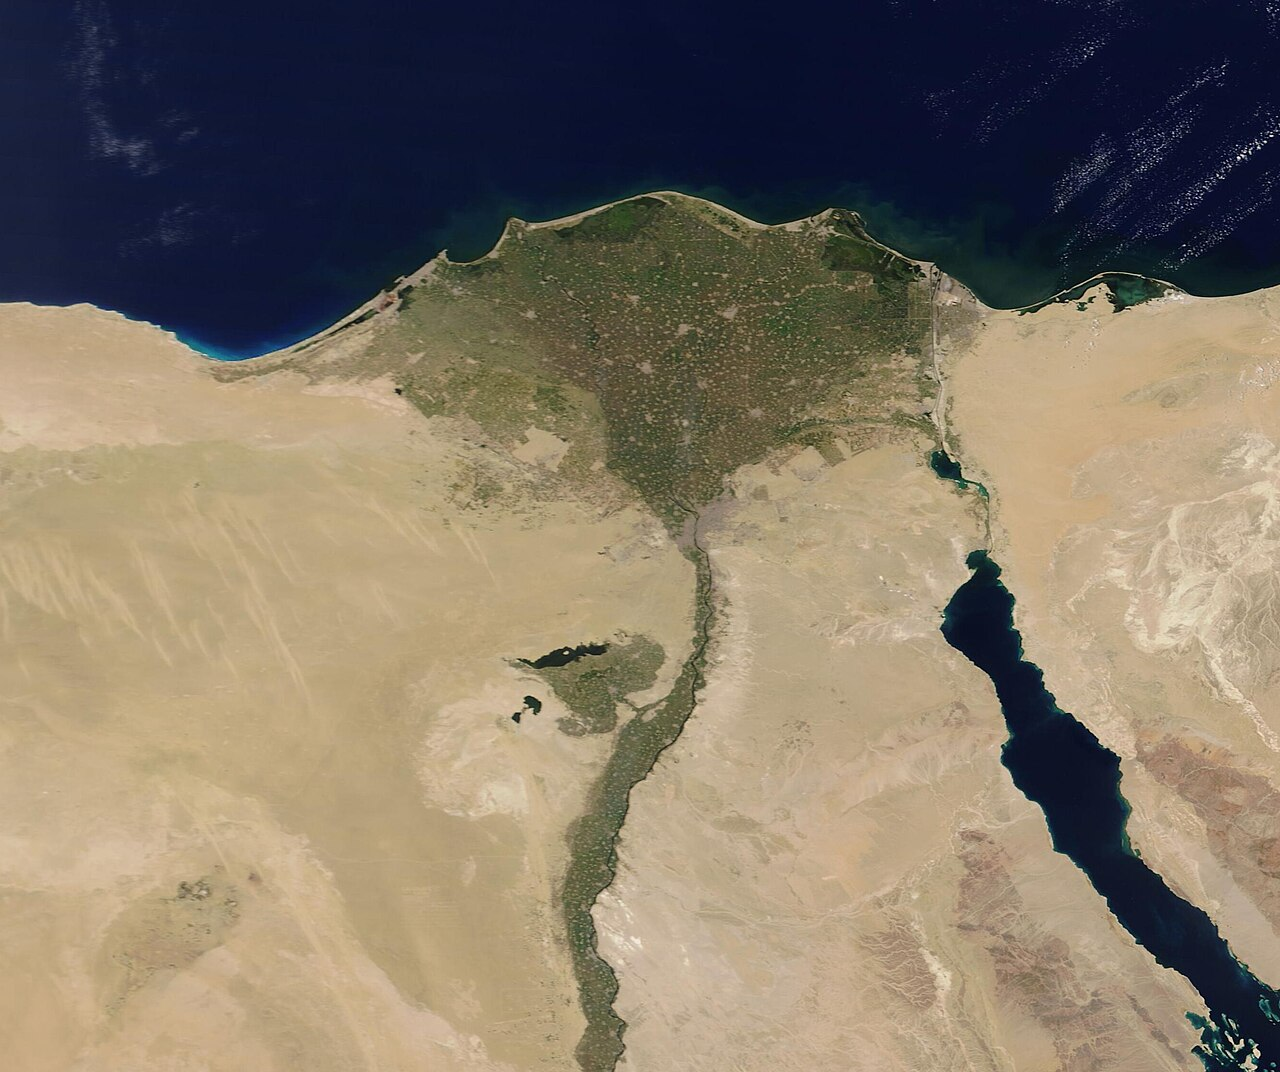
\includegraphics[width=\linewidth]{images/book1/g5-nile-delta-modis.jpg}
\end{minipage}

{\small 左：从上方看的\omterm{def:g5:water-shapes-the-land:delta}{三角洲}，各分支\omterm{def:g5:water-shapes-the-land:deposition}{沉积}的泥和沙
在旧\omterm{def:g1:landscapes-around-us:water}{海岸}之外形成新的陆地。右：埃及尼罗河\omterm{def:g5:water-shapes-the-land:delta}{三角洲}，由卫星拍摄
（海在上方）：绿色的农田呈扇形，铺展在河泥之上，
位于沙漠之中。照片：
NASA，公有领域。}
% ledger: nasa:nile-delta-modis
\end{omfigure}

\section{洪水}

连日降雨，或春季积雪迅速融化时，\omterm{def:g1:landscapes-around-us:water}{河流}
所接收的水量超过了河道的容纳能力。

\begin{definition}[洪水与河漫滩]\label{def:g5:water-shapes-the-land:flood}
\emph{洪水}\index{洪水}是指水淹没了
平时通常干燥的土地。河水涨过河岸，漫向两侧的
平坦土地。这片平地\omterm{def:g1:landscapes-around-us:water}{河流}时常淹没，就是其
\emph{河漫滩}\index{河漫滩}。
\end{definition}

\begin{omfigure}
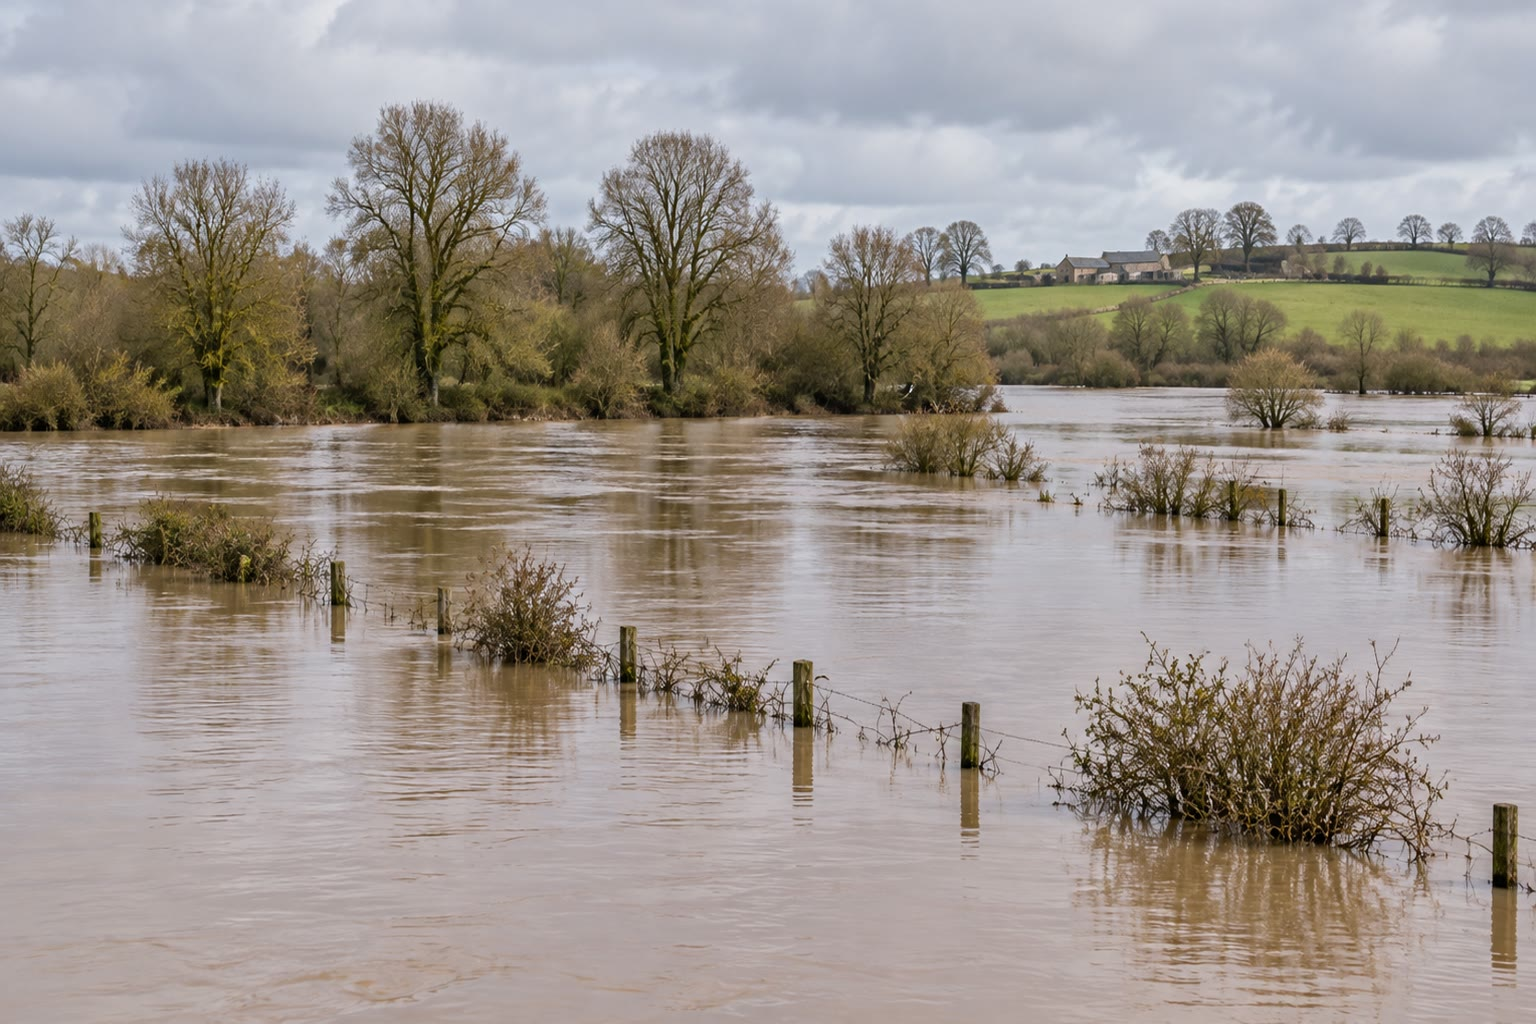
\includegraphics[width=0.5\linewidth]{images/book1/ai/g5-flooded-meadow.jpg}

{\small 连日降雨后，草地被\omterm{def:g5:water-shapes-the-land:flood}{洪水}淹没。沿树木排成的
线标出\omterm{def:g1:landscapes-around-us:water}{河流}平时的河岸；农场位于较高的地面上。}
\end{omfigure}

河水泛滥并非什么反常的事，它只是在做\omterm{def:g1:landscapes-around-us:water}{河流}
一直以来所做的事。\omterm{def:g5:water-shapes-the-land:flood}{河漫滩}是它的领地。事实上，正是\omterm{def:g1:landscapes-around-us:water}{河流}塑造了它：
每次\omterm{def:g5:water-shapes-the-land:flood}{洪水}都会在田野上留下一层薄薄的泥，
这正是\omterm{def:g5:water-shapes-the-land:flood}{河漫滩}土壤如此肥沃的原因。很久以前，埃及
的农民等待尼罗河一年一度的\omterm{def:g5:water-shapes-the-land:flood}{洪水}，\omterm{def:g5:water-shapes-the-land:flood}{洪水}灌溉了他们的田地，
并带来新的\omterm{def:g3:stones-pebbles-sand:sand}{泥沙}。

但是，\omterm{def:g5:water-shapes-the-land:flood}{洪水}对住在\omterm{def:g5:water-shapes-the-land:flood}{河漫滩}上的人十分危险。房屋
可能被水淹没，湍急的\omterm{def:g5:water-shapes-the-land:flood}{洪水}还会冲走
汽车和人。明智的城镇把房屋建在较高处，
把\omterm{def:g5:water-shapes-the-land:flood}{河漫滩}留给农田、草地和公园。在\cref{ch:g5:natural-hazards}中，
我们将看到人们如何应对\omterm{def:g5:water-shapes-the-land:flood}{洪水}并保障安全。

\begin{safety}
切勿在\omterm{def:g5:water-shapes-the-land:flood}{洪水}中行走、骑车或玩耍，也不要靠近发\omterm{def:g5:water-shapes-the-land:flood}{洪水}的
\omterm{def:g1:landscapes-around-us:water}{河流}：水流比看上去更急、更深，还可能掩盖坑洞和敞开的排水口。
请远离，直到负责的大人
认定安全为止。
\end{safety}

\section{练习}

\begin{exercise}[$\star$]\label{exo:g5:water-shapes-the-land:1}
指出下列过程属于\omterm{def:g5:water-shapes-the-land:weathering}{风化}、\omterm{def:g5:water-shapes-the-land:erosion}{侵蚀}还是\omterm{def:g5:water-shapes-the-land:deposition}{沉积}？
\begin{enumerate}
  \item[(a)] 山上\omterm{def:g3:stones-pebbles-sand:rock}{岩石}裂缝中的冰将\omterm{def:g3:stones-pebbles-sand:rock}{岩石}劈开。
  \item[(b)] 发\omterm{def:g5:water-shapes-the-land:flood}{洪水}的\omterm{def:g1:landscapes-around-us:water}{河流}把\omterm{def:g3:stones-pebbles-sand:sand}{沙子}从河岸带走。
  \item[(c)] 平静的湖底\omterm{def:g5:water-shapes-the-land:deposition}{沉积}了一层泥。
  \item[(d)] 树根劈裂了一堵石墙。
\end{enumerate}
\end{exercise}

\begin{exercise}[$\star$]\label{exo:g5:water-shapes-the-land:2}
\omterm{def:g1:landscapes-around-us:water}{河流}的\omterm{def:g5:water-shapes-the-land:source-mouth}{源头}是什么？\omterm{def:g5:water-shapes-the-land:source-mouth}{河口}是什么？\omterm{def:g5:water-shapes-the-land:source-mouth}{支流}是什么？
\end{exercise}

\begin{exercise}[$\star$]\label{exo:g5:water-shapes-the-land:3}
请按从\omterm{def:g5:water-shapes-the-land:source-mouth}{源头}到大海的顺序，排列\omterm{def:g1:landscapes-around-us:water}{河流}的以下部分：
\omterm{def:g5:water-shapes-the-land:meander}{曲流}、\omterm{def:g5:water-shapes-the-land:delta}{三角洲}、狭窄的 V 形\omterm{def:g1:landscapes-around-us:landform}{山谷}和\omterm{def:g5:water-shapes-the-land:source-mouth}{源头}。
\end{exercise}

\begin{exercise}[$\star$]\label{exo:g5:water-shapes-the-land:4}
判断下列说法是否正确，并说明理由。
\begin{enumerate}
  \item[(a)] 坚硬的\omterm{def:g3:stones-pebbles-sand:rock}{岩石}永远不会发生变化。
  \item[(b)] 流速快的\omterm{def:g1:landscapes-around-us:water}{河流}比流速慢的\omterm{def:g1:landscapes-around-us:water}{河流}能搬运更大的石块。
  \item[(c)] 最细的泥先在靠近\omterm{def:g5:water-shapes-the-land:source-mouth}{源头}处\omterm{def:g5:water-shapes-the-land:deposition}{沉积}。
\end{enumerate}
\end{exercise}

\begin{exercise}[$\star$]\label{exo:g5:water-shapes-the-land:5}
下图是从上方俯视的一段河弯。

\begin{center}
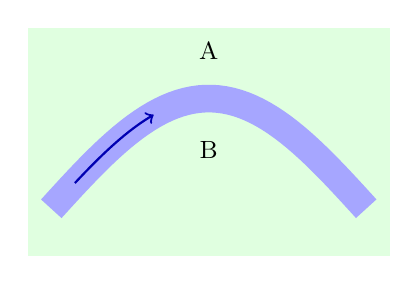
\begin{tikzpicture}[x=1cm, y=1cm, font=\small]
  \fill[green!12] (-0.3,-0.6) rectangle (4.3,2.3);
  \draw[blue!35, line width=10pt] plot[domain=0:4, samples=50]
    (\x,{1.4*sin(\x*45)});
  \draw[blue!70!black, ->, thick] plot[domain=0.3:1.3, samples=20]
    (\x,{1.4*sin(\x*45)});
  \node at (2,2.0) {A};
  \node at (2,0.75) {B};
\end{tikzpicture}
\end{center}
\omterm{def:g1:landscapes-around-us:water}{河流}\omterm{def:g5:water-shapes-the-land:erosion}{侵蚀}土地的是 A 岸还是 B 岸？\omterm{def:g5:water-shapes-the-land:deposition}{沉积}\omterm{def:g3:stones-pebbles-sand:sand}{沙子}的
是哪一岸？
\end{exercise}

\begin{exercise}[$\star$]\label{exo:g5:water-shapes-the-land:6}
在山区，河床上覆盖着大石块；靠近\omterm{def:g2:water-on-earth:ocean}{海洋}时，
河床上则覆盖着沙和泥。这是为什么？
\end{exercise}

\begin{exercise}[$\star\star$]\label{exo:g5:water-shapes-the-land:7}
一条河长 600 千米。其上游占全长的前
$\frac{1}{6}$，中游占接下来的
$\frac{1}{2}$。
\begin{enumerate}
  \item[(a)] 上游长多少？中游呢？
  \item[(b)] 下游长多少？它占全河的
        几分之几？
\end{enumerate}
\end{exercise}

\begin{exercise}[$\star\star$]\label{exo:g5:water-shapes-the-land:8}
再看一看从空间站拍摄的马莫雷河照片，
见第~\pageref{fig:g5:water-shapes-the-land:mamore}~页。河弯内侧的浅色斑块是什么？
河边那些深色弯曲的\omterm{def:g1:landscapes-around-us:water}{湖泊}是什么？它们是如何形成的？
\end{exercise}

\begin{exercise}[$\star\star$]\label{exo:g5:water-shapes-the-land:9}
某镇想在河边平坦的绿色草地上建一所新学校，
因为那里地势平坦且便宜。你会对镇议会说些什么？
请使用词语\emph{\omterm{def:g5:water-shapes-the-land:flood}{洪水}}和\emph{\omterm{def:g5:water-shapes-the-land:flood}{河漫滩}}。
\end{exercise}

\begin{exercise}[$\star\star$]\label{exo:g5:water-shapes-the-land:10}
世界上的\omterm{def:g1:landscapes-around-us:water}{河流}每年向大海输送约
120 亿吨\omterm{def:g3:stones-pebbles-sand:sand}{泥沙}。
\begin{enumerate}
  \item[(a)] 平均每月是多少吨？
  \item[(b)] 一辆大货车可载 10 吨。要运走一个月的\omterm{def:g3:stones-pebbles-sand:sand}{泥沙}，
        需要多少车次？
\end{enumerate}
\end{exercise}

\begin{exercise}[$\star\star\star$]\label{exo:g5:water-shapes-the-land:11}
讲一讲一粒\omterm{def:g3:stones-pebbles-sand:sand}{沙子}的故事。它起初是高山上\omterm{def:g3:stones-pebbles-sand:rock}{岩石}的一部分，
许多年后，它最终停留在\omterm{def:g5:water-shapes-the-land:delta}{三角洲}中。请使用词语
\emph{\omterm{def:g5:water-shapes-the-land:weathering}{风化}}、\emph{\omterm{def:g5:water-shapes-the-land:erosion}{侵蚀}}和\emph{\omterm{def:g5:water-shapes-the-land:deposition}{沉积}}，并说明这粒\omterm{def:g3:stones-pebbles-sand:sand}{沙子}
在\omterm{def:g1:landscapes-around-us:water}{河流}的上游、中游和下游各经历了什么。
\end{exercise}
